\graphicspath{{sections/visualize/images/}}
\section[Workspace]{Workspace \myAuthor{Lucas Schlager / Christoph Schwarz}}
Die Entwicklungsumgebung wurde mithilfe von Docker und Devcontainer realisiert. Diese Herangehensweise bietet mehrere Vorteile, darunter das Einsparen von Ressourcen, da keine virtuelle Maschine aufgesetzt werden muss. 

Ein bedeutender Vorteil der Nutzung von Docker für diesen Use Case ist die Konsistenz der Entwicklungsumgebungen. Unabhängig davon, auf welchem Rechner das Projekt bearbeitet wird, kann durch das standardisierte Docker-Image eine identische Umgebung geschaffen werden, die überall gleich läuft. Dies minimiert Kompatibilitätsprobleme und erleichtert die Zusammenarbeit im Team erheblich. Zudem ermöglicht Docker eine einfache Skalierung und Verwaltung von Abhängigkeiten, was besonders in größeren Projekten von Vorteil ist.

Die aktuelle Umgebung kann immer mit einem einfachen `docker pull` aktualisiert werden. Das Docker-Image wird bei einer Änderung mit Hilfe der GitLab CI gebaut und auf die GitLab Registry hochgeladen. Über eine `devcontainer.json` konnte zusätzlich die IDE, in diesem Fall VSCode, mit Plugins konfiguriert werden.

Eine Herausforderung bestand darin, GUI-Anwendungen aus dem Docker-Image auf das Host-System zu pipen. Dies war unter Linux weniger aufwendig, jedoch hatten wir unter Windows einige Probleme. Diese konnten jedoch mit verschiedenen Skripten und Programmen gelöst werden, sodass unsere Entwicklungsumgebung sowohl unter Windows als auch unter Linux einwandfrei funktioniert.

\section{Visualizer}
\subsection{Was war das zu lösende Problem?}
Die Anforderungen an das Teilmodul umfassten das Modellieren und Texturieren des Puzzles, die Beweglichkeit des Roboters zu gewährleisten sowie die korrekte Anordnung seiner Einzelteile. Zusätzlich war die Entwicklung der Logik erforderlich, die das Aufnehmen und Ablegen der Puzzleteile steuert.\\
\\
Zusätzlich stellten wir den Workspace für die Entwicklung dieser wurde unter verwendung von Docker und Devcontainer in VSCode realisiert.\\

\subsection{Was haben wir gemacht? / Wie haben wir die Lösungen umgesetzt / Implementierung}
Zu Beginn unseres Projekts bestand unser erstes Ziel darin, einen einheitlichen Workspace für das gesamte Team zu schaffen, um zu verhindern, dass bei der Integration der Arbeit Unterschiede in den Standardkonfigurationen Probleme verursachen. Ein einheitlicher Workspace, der automatisch alle notwendigen Abhängigkeiten installiert, vereinfacht zudem den Entwicklungsprozess. Die Docker-Container wurden mit Hilfe von GitLab CI/CD erstellt und in die GitLab Docker-Registry hochgeladen, von wo aus sie dann von allen Projektteilnehmern über die \texttt{devcontainer.json} heruntergeladen werden konnten. Eine Herausforderung bestand darin, UI-Programme aus Docker heraus zu pipen, sodass das Fenster auf dem Host-Rechner angezeigt wird. Auf Linux-Systemen war dies weniger problematisch, jedoch traten anfangs Schwierigkeiten unter Windows auf, die jedoch ebenfalls gelöst wurden.\\
\\
Nachdem der Workspace eingerichtet war, konnten wir uns den ersten Aufgaben der 3D-Visualisierung widmen. Zunächst integrierten wir den Roboter in Coin3D. Dazu wurden mehrere sogenannte IV-Dateien, die jeweils einen Arm des Roboters enthalten, durch Imports in eine große IV-Datei zusammengefügt. An jedes Import-Statement fügten wir die Transformationen der DH-Parameter des Control-Teams ein. Als der Roboter anschließend nicht mehr korrekt zusammenpasste, positionierten wir die einzelnen Arme neu, sodass der Roboter als ein zusammenhängendes Objekt im 3D-Viewer existiert (Figure \ref{fig:Kuka_KR6}). Zusätzlich implementierten wir Transformationen, die es dem Roboter ermöglichen, sich realitätsgetreu über seine Gelenke zu bewegen. Durch die Trennung der einzelnen Arme mittels eines \texttt{SoSeparator} und das Einfügen der Transformationen kann nun über eine \texttt{SoSearchOperation} der Knoten im Programm gefunden werden, was die Animation des Roboters ermöglicht.\\
\\
Nachdem der Roboter fertiggestellt und beweglich gemacht wurde, konnten wir uns unserem nächsten Projektziel zuwenden, die erstellung des Puzzelteils. Zuerst führten wir einen Test durch, um die Leistungsfähigkeit von Coin3D in einem Container mit zahlreichen Texturen zu testen. Für diesen Test platzierten wir 1000 unterschiedliche Bilder auf Objekten und führten ein Rendering durch. Das Ergebnis war positiv, da der 3D-Viewer weiterhin flüssig und ohne Verzögerungen bedient werden konnte.\\
\\
Vom Solver-Team erhalten wir eine PNG-Datei (Textur des Puzzles) und eine SVG-Datei (Kontur des Puzzles), die in ein dreidimensionales Objekt umgewandelt werden müssen. Dazu laden wir zunächst die Punkte der Kontur in Coin3D mittels eines \texttt{SoCoordinate3}-Objekts. Um das dreidimensionale Puzzle zu erstellen, werden dieselben Punkte erneut, jedoch mit einem Höhenoffset, ins Programm geladen. Da das SVG lediglich die Kontur abbildet und die Mitte des Puzzles keine Punkte enthält, ist es notwendig, die Kontur zu triangulieren. Dies erfolgt mit Hilfe der Bibliothek Poly2Tri.\\
Anschließend wurde die Textur mit Hilfe eines \texttt{SoTexture}-Objekts auf das Puzzle-Teil aufgetragen. Nachdem die Koordinaten in der SVG-Datei mit den Pixeln in der PNG-Datei abgeglichen wurden, können wir nun die Textur präzise über das dreidimensionale Objekt legen (Figure \ref{fig:Puzzle}). Danach wird noch der Mittelpunkt des Puzzelteils auf den Bildmittelpunkt des PNG gesetzt, da dies notwendig für die anderen Teams war.\\
\\
\textbf{Schnittstellen implementierung:}
\begin{enumerate}
    \item \textit{/control/angles} Über diese node werden die Bewegungen so wie das Ablegen und Aufnehmen eines Puzzelteils an den Roboter gesendet.
    \item \textit{/digitalize/imgs} Über diese node werden die Puzzelteile als 3D-Objekt gebaut und in eine Map geladen.
    \item \textit{/solver/startpos} Über diese node werden die Puzzelteile initial an den mitgegebenen Koordinaten im 3D-Raum eingefügt. 
\end{enumerate}
Nachdem es möglich war den Roboter anzuzeigen und zu bewegen, ein Puzzelteile aus Punkten und einem PNG zu erstellen, haben wir uns an die Schnittstellen implementierung gesetzt. Zuerst haben wir hierfür die Schnittstelle \textbf{\textit{"/control/angles"}} implementiert. Diese ist dafür zuständig den Roboter zu bewegen. Dafür mussten wir eine callback Methode implementieren, welche die neuen Winkel in Radiant in ein Array speichert. Dieses musste von einem Mutex geschützt werden, da es sonst passieren kann, dass der SoIdelSensor im selben Moment auf das Array zugreift. Der SoIdleSensor wurde für alle Schnittstellen implementiert. Dieser stellt sicher, dass Änderungen am Szenegraphen nur dann geschehen, wenn sich dieser im Idle-Zustand befindet. Wenn dieser Aufgerufen wird, wird die Methode \textbf{\textit{set\_rotation\_angle\_robot()}} ausgeführt, welche dann die Winkel aller Arme neu setzt. Dies geschieht wie zuvor schon erwähnt über eine SoSearch und der Transformationsanwendung auf diese.\\
\\
Die nächste Schnittstelle ist die \textbf{\textit{"/digitalize/imgs"}}, aus welcher die Punkte und PNG´s der einzelnen Puzzelteile geholt werden. Aus dieser message werden die Puzzelteile dann verarbeitet und an einen SoSeperator gehangen. Diese werden dann in einer map mit key: id und value: SoSeperator* gespeichert.\\
Die Schnittstelle \textbf{\textit{"/solver/startpos"}} wird dann subscribed um die Startpositionen der einzelnen Puzzelteile zu bekommen. Diese werden so übergeben, dass aus diesen die Position und die Translation im Raum auf das Puzzelteil angewendet werden kann.\\
\\
Die letzte zu implementierende Schnittstelle war die \textbf{\textit{"/control/puzzlebool"}}. Diese Schnittstelle ist dafür da mittzuteilen, ob ein Puzzelteil aufgehoben oder abgelegt werden soll. Dies geschieht über einen mitgegebenen boolean (true=pick, false=drop) und der ID des Puzzelteils. Hierfür gibt es zwei Fälle:
\begin{enumerate}
    \item Fall (true=pick): Hier wird das zu nehmende Puzzelteil aus der map geladen und seine aktuelle Transformation wird gelöscht. Danach wird es an den SoSeperator des Roboter gehangen und bewegt sich dadurch mit.
    \item Fall (false=drop): Hier wird die aktuelle Position des Puzzelteils über eine SoSearchAction und eine darauffolgende SoGetMatrixAction ermittelt. Sobald diese ermittelt ist, wird das Puzzelteil aus dem SoSeperator des Roboter gelöscht und dem root SoSeperator wieder hinzugefügt. Davor wird allerdings noch die vorher ermittelte Transformation auf den SoSeperator des Puzzelteils angewendet.
\end{enumerate}
Um den Zeitpunkt, wann das Puzzelteil abgelegt werden soll, besser mit der Schnittstelle \textbf{\textit{/control/angles}} zu verbinden, wurden die beiden ros nodes zu einer Zusamengefasst. Der Grund liegt hierbei daran, dass wenn die node \textbf{\textit{/control/puzzlebool}} gesendet wurde, es sein kann, dass der Roboter sich durch die node \textbf{\textit{/control/angles}} schon wieder weiterbewegt hat und dadurch das Puzzelteil nicht genau dort liegt wo es soll. Da nun der boolean Wert mit der \textbf{\textit{/control/angles}} node gesendet wird, wird dieser Fehler behohben. Auch mögliche verluste von Nachrichten sind dadurch behoben, da boolean=true nun bedeutet, dass ein Puzzle attached ist und dieser Wert erst wieder auf false wechselt, wenn das Puzzle abgelgt werden soll.\\
\\
Durch das Zusammenspiel der einzelnen Schnittstellen und der Implementierung der Visualisierung ist es nun also möglich:
\begin{enumerate}
    \item Den Roboter zu laden.
    \item Die Puzzelteile, nachdem diese per ros verschickt wurden als 3D-Objekte zu laden.
    \item Die Puzzelteile an ihren Startpositionen zu platzieren.
    \item Den Roboter an die gewünschte Stelle zu bewegen.
    \item Ein Puzzelteil mit dem Roboter aufzuheben und mit dem Roboter mitzubewegen.
    \item Ein Puzzelteil and er Stelle ab zu setzen, an der der Roboter sich gerade befindet.
\end{enumerate}
Dadurch ist es möglich die komplette Lösung eines beliebigen Puzzles über die Schnittstellen der ros2 nodes darzustellen.
\begin{figure}[H]
    \centering
    \begin{subfigure}[b]{0.45\textwidth}
        \centering
        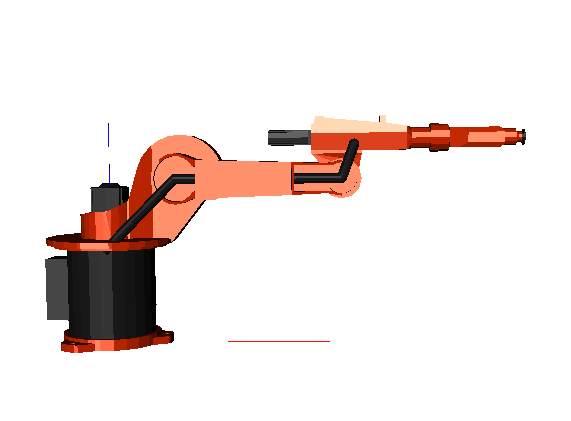
\includegraphics[width=\textwidth]{kuka_kr6.png}
        \caption{Visualisierte Roboter in Coin3D über .iv-Files}
        \label{fig:Kuka_KR6}
    \end{subfigure}
    \hfill
    \begin{subfigure}[b]{0.45\textwidth}
        \centering
        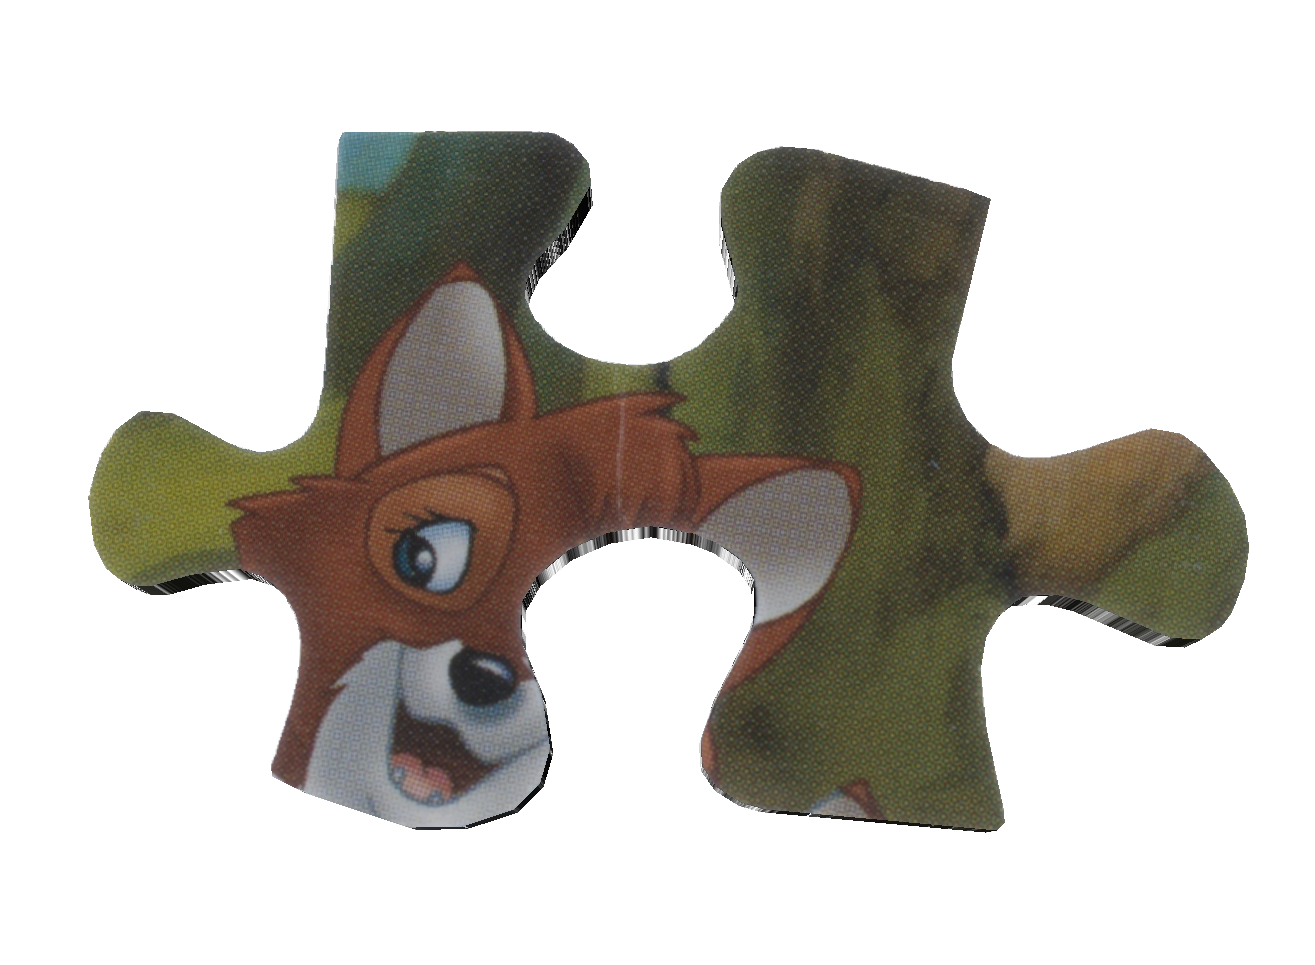
\includegraphics[width=\textwidth]{puzzle.png}
        \caption{3D-Objekt eines Puzzelteils}
        \label{fig:Simulated-Test-environment}
    \end{subfigure}
    \caption{3D-Objekte des Roboters und eines Puzzelteils}
    \label{fig:Puzzle}
\end{figure}